\documentclass[twoside]{book}

% Packages required by doxygen
\usepackage{fixltx2e}
\usepackage{calc}
\usepackage{doxygen}
\usepackage{graphicx}
\usepackage[utf8]{inputenc}
\usepackage{makeidx}
\usepackage{multicol}
\usepackage{multirow}
\PassOptionsToPackage{warn}{textcomp}
\usepackage{textcomp}
\usepackage[nointegrals]{wasysym}
\usepackage[table]{xcolor}

% Font selection
\usepackage[T1]{fontenc}
\usepackage{mathptmx}
\usepackage[scaled=.90]{helvet}
\usepackage{courier}
\usepackage{amssymb}
\usepackage{sectsty}
\renewcommand{\familydefault}{\sfdefault}
\allsectionsfont{%
  \fontseries{bc}\selectfont%
  \color{darkgray}%
}
\renewcommand{\DoxyLabelFont}{%
  \fontseries{bc}\selectfont%
  \color{darkgray}%
}
\newcommand{\+}{\discretionary{\mbox{\scriptsize$\hookleftarrow$}}{}{}}

% Page & text layout
\usepackage{geometry}
\geometry{%
  a4paper,%
  top=2.5cm,%
  bottom=2.5cm,%
  left=2.5cm,%
  right=2.5cm%
}
\tolerance=750
\hfuzz=15pt
\hbadness=750
\setlength{\emergencystretch}{15pt}
\setlength{\parindent}{0cm}
\setlength{\parskip}{0.2cm}
\makeatletter
\renewcommand{\paragraph}{%
  \@startsection{paragraph}{4}{0ex}{-1.0ex}{1.0ex}{%
    \normalfont\normalsize\bfseries\SS@parafont%
  }%
}
\renewcommand{\subparagraph}{%
  \@startsection{subparagraph}{5}{0ex}{-1.0ex}{1.0ex}{%
    \normalfont\normalsize\bfseries\SS@subparafont%
  }%
}
\makeatother

% Headers & footers
\usepackage{fancyhdr}
\pagestyle{fancyplain}
\fancyhead[LE]{\fancyplain{}{\bfseries\thepage}}
\fancyhead[CE]{\fancyplain{}{}}
\fancyhead[RE]{\fancyplain{}{\bfseries\leftmark}}
\fancyhead[LO]{\fancyplain{}{\bfseries\rightmark}}
\fancyhead[CO]{\fancyplain{}{}}
\fancyhead[RO]{\fancyplain{}{\bfseries\thepage}}
\fancyfoot[LE]{\fancyplain{}{}}
\fancyfoot[CE]{\fancyplain{}{}}
\fancyfoot[RE]{\fancyplain{}{\bfseries\scriptsize Generated on Wed Jun 8 2016 20\+:23\+:02 for My Project by Doxygen }}
\fancyfoot[LO]{\fancyplain{}{\bfseries\scriptsize Generated on Wed Jun 8 2016 20\+:23\+:02 for My Project by Doxygen }}
\fancyfoot[CO]{\fancyplain{}{}}
\fancyfoot[RO]{\fancyplain{}{}}
\renewcommand{\footrulewidth}{0.4pt}
\renewcommand{\chaptermark}[1]{%
  \markboth{#1}{}%
}
\renewcommand{\sectionmark}[1]{%
  \markright{\thesection\ #1}%
}

% Indices & bibliography
\usepackage{natbib}
\usepackage[titles]{tocloft}
\setcounter{tocdepth}{3}
\setcounter{secnumdepth}{5}
\makeindex

% Hyperlinks (required, but should be loaded last)
\usepackage{ifpdf}
\ifpdf
  \usepackage[pdftex,pagebackref=true]{hyperref}
\else
  \usepackage[ps2pdf,pagebackref=true]{hyperref}
\fi
\hypersetup{%
  colorlinks=true,%
  linkcolor=blue,%
  citecolor=blue,%
  unicode%
}

% Custom commands
\newcommand{\clearemptydoublepage}{%
  \newpage{\pagestyle{empty}\cleardoublepage}%
}


%===== C O N T E N T S =====

\begin{document}

% Titlepage & ToC
\hypersetup{pageanchor=false,
             bookmarks=true,
             bookmarksnumbered=true,
             pdfencoding=unicode
            }
\pagenumbering{roman}
\begin{titlepage}
\vspace*{7cm}
\begin{center}%
{\Large My Project }\\
\vspace*{1cm}
{\large Generated by Doxygen 1.8.8}\\
\vspace*{0.5cm}
{\small Wed Jun 8 2016 20:23:02}\\
\end{center}
\end{titlepage}
\clearemptydoublepage
\tableofcontents
\clearemptydoublepage
\pagenumbering{arabic}
\hypersetup{pageanchor=true}

%--- Begin generated contents ---
\chapter{Namespace Index}
\section{Namespace List}
Here is a list of all documented namespaces with brief descriptions\+:\begin{DoxyCompactList}
\item\contentsline{section}{\hyperlink{namespace_cristian_algo_client}{Cristian\+Algo\+Client} }{\pageref{namespace_cristian_algo_client}}{}
\end{DoxyCompactList}

\chapter{Hierarchical Index}
\section{Class Hierarchy}
This inheritance list is sorted roughly, but not completely, alphabetically\+:\begin{DoxyCompactList}
\item \contentsline{section}{Cristian\+Interface}{\pageref{interface_cristian_interface}}{}
\begin{DoxyCompactList}
\item \contentsline{section}{Cristian}{\pageref{class_cristian}}{}
\end{DoxyCompactList}
\item Marshal\+By\+Ref\+Object\begin{DoxyCompactList}
\item \contentsline{section}{Cristian}{\pageref{class_cristian}}{}
\end{DoxyCompactList}
\item \contentsline{section}{Cristian\+Algo\+Server.\+Server}{\pageref{class_cristian_algo_server_1_1_server}}{}
\end{DoxyCompactList}

\chapter{Class Index}
\section{Class List}
Here are the classes, structs, unions and interfaces with brief descriptions\+:\begin{DoxyCompactList}
\item\contentsline{section}{\hyperlink{class_cristian_algo_client_1_1_client}{Cristian\+Algo\+Client.\+Client} \\*Klasa zawiera obsługę algorytmu Cristiana ze strony klienta }{\pageref{class_cristian_algo_client_1_1_client}}{}
\item\contentsline{section}{\hyperlink{interface_cristian_interface}{Cristian\+Interface} \\*Wspólny interfejs }{\pageref{interface_cristian_interface}}{}
\end{DoxyCompactList}

\chapter{Namespace Documentation}
\hypertarget{namespace_cristian_algo_server}{\section{Package Cristian\+Algo\+Server}
\label{namespace_cristian_algo_server}\index{Cristian\+Algo\+Server@{Cristian\+Algo\+Server}}
}
\subsection*{Classes}
\begin{DoxyCompactItemize}
\item 
class \hyperlink{class_cristian_algo_server_1_1_server}{Server}
\begin{DoxyCompactList}\small\item\em Klasa zawiera obsługę zadań wykonywanych przez serwer w algorytmie Cristiana. \end{DoxyCompactList}\end{DoxyCompactItemize}

\chapter{Class Documentation}
\hypertarget{class_cristian}{\section{Cristian Class Reference}
\label{class_cristian}\index{Cristian@{Cristian}}
}


Klasa dziedzicząca po interfejsie i klasie Marshal\+By\+Ref\+Object, która pozwala na dostęp do klasy z poza domeny danej aplikacji Klasa zawiera implementacje funkcji zlecanej do wykonania przez serwer.  


Inheritance diagram for Cristian\+:\begin{figure}[H]
\begin{center}
\leavevmode
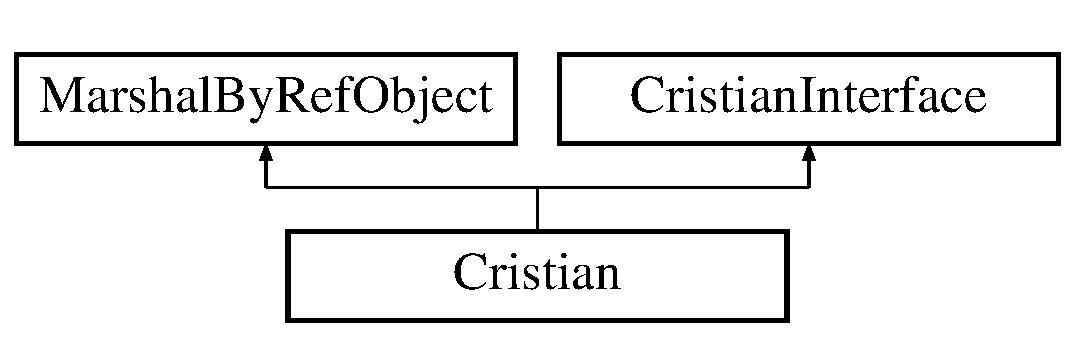
\includegraphics[height=2.000000cm]{class_cristian}
\end{center}
\end{figure}
\subsection*{Public Member Functions}
\begin{DoxyCompactItemize}
\item 
Date\+Time \hyperlink{class_cristian_a15a9f71968248b89a6f4c609651ad5a0}{Get\+Server\+Time} ()
\begin{DoxyCompactList}\small\item\em metoda wysyłająca do klienta akualny czas serwera \end{DoxyCompactList}\end{DoxyCompactItemize}


\subsection{Detailed Description}
Klasa dziedzicząca po interfejsie i klasie Marshal\+By\+Ref\+Object, która pozwala na dostęp do klasy z poza domeny danej aplikacji Klasa zawiera implementacje funkcji zlecanej do wykonania przez serwer. 

\subsection{Member Function Documentation}
\hypertarget{class_cristian_a15a9f71968248b89a6f4c609651ad5a0}{\index{Cristian@{Cristian}!Get\+Server\+Time@{Get\+Server\+Time}}
\index{Get\+Server\+Time@{Get\+Server\+Time}!Cristian@{Cristian}}
\subsubsection[{Get\+Server\+Time}]{\setlength{\rightskip}{0pt plus 5cm}Date\+Time Cristian.\+Get\+Server\+Time (
\begin{DoxyParamCaption}
{}
\end{DoxyParamCaption}
)\hspace{0.3cm}{\ttfamily [inline]}}}\label{class_cristian_a15a9f71968248b89a6f4c609651ad5a0}


metoda wysyłająca do klienta akualny czas serwera 

aktualny czas serwera 

Implements \hyperlink{interface_cristian_interface}{Cristian\+Interface}.



The documentation for this class was generated from the following file\+:\begin{DoxyCompactItemize}
\item 
Program.\+cs\end{DoxyCompactItemize}

\hypertarget{interface_cristian_interface}{\section{Cristian\+Interface Interface Reference}
\label{interface_cristian_interface}\index{Cristian\+Interface@{Cristian\+Interface}}
}


Wspólny interfejs.  


\subsection*{Public Member Functions}
\begin{DoxyCompactItemize}
\item 
\hypertarget{interface_cristian_interface_a85bc7efa032f0cedfad7476ff9a644f3}{Date\+Time {\bfseries Get\+Server\+Time} ()}\label{interface_cristian_interface_a85bc7efa032f0cedfad7476ff9a644f3}

\end{DoxyCompactItemize}


\subsection{Detailed Description}
Wspólny interfejs. 

The documentation for this interface was generated from the following file\+:\begin{DoxyCompactItemize}
\item 
Program.\+cs\end{DoxyCompactItemize}

\hypertarget{class_cristian_algo_server_1_1_server}{\section{Cristian\+Algo\+Server.\+Server Class Reference}
\label{class_cristian_algo_server_1_1_server}\index{Cristian\+Algo\+Server.\+Server@{Cristian\+Algo\+Server.\+Server}}
}


Klasa zawiera obsługę zadań wykonywanych przez serwer w algorytmie Cristiana.  




\subsection{Detailed Description}
Klasa zawiera obsługę zadań wykonywanych przez serwer w algorytmie Cristiana. 

Zadania serwera\+:
\begin{DoxyItemize}
\item tworzenie połączenia, (ustawienie protokołu i rejestracja kanału)
\item oczekiwanie na połączenie klienta
\item wykonanie żądanego zadania
\item odesłanie otrzymanych wyników do klienta 
\end{DoxyItemize}

The documentation for this class was generated from the following file\+:\begin{DoxyCompactItemize}
\item 
Program.\+cs\end{DoxyCompactItemize}

%--- End generated contents ---

% Index
\newpage
\phantomsection
\addcontentsline{toc}{chapter}{Index}
\printindex

\end{document}
